 \newcommand{\pwd}{key}

\renewcommand{\password}{key\xspace}

We introduce the problem  through an example, and outline our
approach.  We work with a  small, class-based object-oriented, sequential language similar to Joe-E \cite{JoeE} with modules,   module-private fields
({accessible} only from   methods {from} the same module),
and unforgeable, un-enumerable addresses.
We distinguish between  \emph{\internalO  objects} --- instances of our internal module $M$'s classes ---
and \emph{\externalO  objects} defined in
\emph{any} number of external modules $\overline M$.%
\!\footnote{We use the notation $\overline z$ for a sequence of $z$, \ie for $z_1,z_2,...z_n$ }
%Program states whose receiver (\prg{this}) is internal are \emph{internal states} -- they are executing code from the internal module -- the other states are  \emph{external states}.
{\prg{Private} methods  {may only be} called by objects of the same
  module,  while \prg{public}  methods  may be {called} by \emph{any}
  object with a reference to the method receiver, {and with
  actual arguments of  dynamic types that match} the declared formal parameter types.}%
\!\footnote{As in Joe-E, we leverage  module-based privacy to restrict propagation of capabilities, and reduce the need for reference monitors etc, \cf Sect 3 in  \cite{JoeE}.}   

\label{s:concepts}
 
We are concerned with guarantees made in an \emph{open} setting; % thatis, 
Our internal module
$M$ must be programmed so that 
  execution of $M$  together with \emph{any} unknown, arbitrary, external modules $\overline M$
% it was "its execution, together ... "SD thinks that the comma  was misleading
will satisfy these guarantees --
%$M$ must ensure these guarantees are satisfied
%These guarantees must  satisfied whenever the $\overline M$  \emph{\externalM} modules are executing, yet 
without relying on any assumptions about $\overline M$'s code.\footnote{This is a critical distinction from e.g.\
cooperative approaches such as rely/guarantee
\cite{relyGuarantee-HayesJones-setss2017,relyGuarantee-vanStaden-mpc2015}.}
All we can rely on, is the guarantee that external code interacts with the internal code only through public methods; such a guarantee may be given by the programming language or by the underlying platform.\footnote{Thus our approach is also applicable to inter-language safety.}
% SD chopped the next sentence. Because I think that  the uninformed reader will be surpised, and the knowledgeable reader will find out soon enough
% The internal module may break these guarantees temporarily,
% so long as they {are reestablished} before (re)entry to an external module.
  
 

\subsection*{\prg{Shop} -- illustrating limited effects}  
\label{sec:how}
\label{sec:shop}

Consider the following internal module \Mshop, % which also includes the 
%containing 
with classes \prg{Item}, \prg{Shop}, \prg{Account}, and \prg{Inventory}. 
Classes \prg{Inventory} and \prg{Item} are straightforward: we elide
their details. 
\prg{Account}s hold a balance and have a \password. 
Access to an \prg{Account},  allows one  to pay money into it, 
and  access to an \prg{Account}  and its \prg{Key}, allows one to withdraw money from it.
A \prg{Shop} has an \prg{Account},
and a public method \prg{buy} to allow a 
\prg{buyer} --- an \prg{external}   object --- to buy
and pay for an \prg{Item}:
 
 % SD chopped  with a method { \prg{pay}.}} 


\begin{lstlisting}[mathescape=true, language=Chainmail, frame=none]
module M$_{shop}$
  ...   
  class Shop
    field accnt:Account, invntry:Inventory, clients:external     
     
    public method buy(buyer:external, anItem:Item)
      int price = anItem.price
      int oldBlnce = this.accnt.blnce
      $\red{\mbox{buyer.pay(this.accnt, price)}}$      
      if (this.accnt.blnce == oldBlnce+price)  
         this.send(buyer,anItem)
      else
         buyer.tell("you have not paid me") 
                       
    private method send(buyer:external, anItem:Item)  
       ...         
\end{lstlisting}
 
 
 
\begin{wrapfigure}[12]{r}{0cm}%expand to fit figure
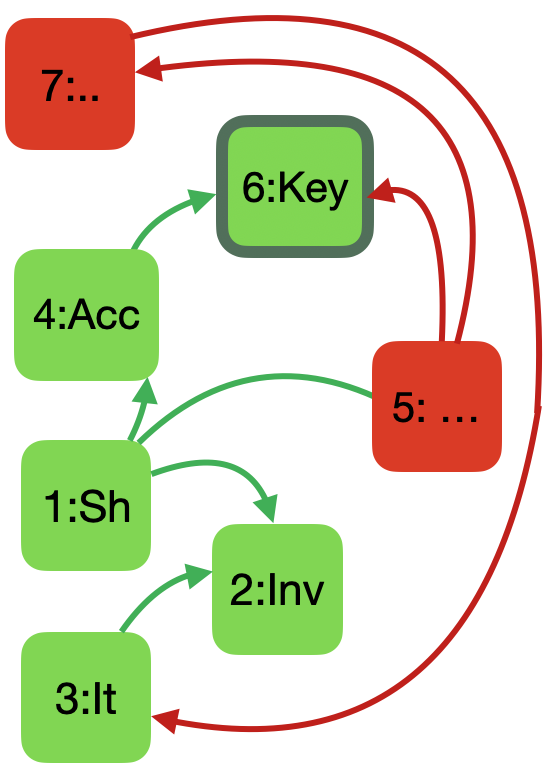
\includegraphics[width=25mm]{diagrams/ShopAtrimmed.png}
\end{wrapfigure}



\noindent The sketch to the right shows a possible heap snippet.
External objects are red; internal objects are green.
%
Each object has a number,
followed by an abbreviated class name: $o_1$, $o_2$ and $o_5$ are a \prg{Shop}, an \prg{Inventory}, and an external object. 
Curved arrows
indicate field values: $o_1$ has three fields, pointing to 
$o_4$, $o_5$ and $o_2$.
%
Fields denote direct access. The transitive closure of direct access
gives indirect (transitive) access: $o_1$ has direct access to $o_4$, and indirect access to $o_6$.
%
Object $o_6$ ---
highlighted with a dark outline
---
is the key capability that allows withdrawal from $o_4$.

The critical point in our code is the external call on line 8,   where the \prg{Shop} asks the \prg{buyer} to pay the price of that item,
by calling  \prg{pay} on \prg{buyer} and passing the \prg{Shop}'s account as an argument.
As \prg{buyer} is an external object, the module \Mshop has no method specification for \prg{pay}, and no 
certainty about what its implementation might do. 


What are the possible effects of that external call?
At line 9, the \prg{Shop} hopes
the buyer will have deposited the price into its account, 
but needs to be certain the \prg{buyer} cannot
%use this %opportunity to access the
%shop's account to drain its money.
have emptied that account instead. 
%
Can the \prg{Shop}  be certain? Indeed, if

\vspace{.05cm}
\begin{enumerate}[(A)]
\item   Prior to the call of  \prg{buy}, the \prg{buyer}  has no eventual access to the account's \password, \ \ \ \emph{----} and
\item  \Mshop ensures that 
\begin{enumerate}[(a)]
\item access to keys is not leaked to external objects, \ \ \ \emph{----} and
\item   funds cannot be withdrawn unless the external entity responsible for the withdrawal (eventually) has  access to the account's \password,
\end{enumerate}
\item[--- then]
\item  The external  call on line 8 can never result in a decrease in the shop's account balance.
\end{enumerate}


 \noindent
The remit of this paper is to provide specification and verification tools that support arguments like the one above.
This gives rise to the following two challenges:\  1$^{st}$:  A specification language which describes access to capabilities and limited effects,\ 
2$^{nd}$: A  Hoare Logic for adherence to such specifications.




%\vspace{.2cm}
%\noindent
% \textbf{NOTE}  \sdN{Replacing the argument by a wrapper to the account which allows payments but forbids withdrawals,    would be ineffectual in \taming} the  effects on line 9. 
%What  if the   \prg{buyer} had access to the account and its \password  \emph{before} the call to \prg{pay}? 
%\se{I don't understand the point here. Are you saying a wrapper might prevent a buyer who has legitimate access to an account from getting it?}
%\sdN{SD: The point I am trying to make is that: \  if before the call to \prg{pay}, the \prg{buyer} had access to the account and its keyword, and when we call \prg{pay} instead of 
%\prg{this.accnt} we pass the wrapper, then the \prg{buyer} would still be able to steal money from \prg{this.accnt}.
%Does this make sense? Shall we drop that point?}
 
 
\subsection{1$^{st}$ Challenge: Specification Language} 

We want to give a formal meaning to the guarantee that for some effect, $E$, and an object $o_c$ which is the capability for $E$:

\vspace{.05cm}

  \begin{minipage}{.05\textwidth}
   \textbf{(*)}
\end{minipage}
\hfill
\begin{minipage}{.95\textwidth}
\begin{flushleft}
$E$  (\eg the account's balance decreases)  can be caused only  by external objects calling methods on internal objects, \\
and only if the causing object has access  to $o_c$ (\eg the key).
\end{flushleft}
\end{minipage}

\vspace{.05cm}

%\begin{quote}
%(*)   \ \ \ \ \ $E$ can be caused only  by external objects calling methods on internal objects, \\
%$\strut \ $ \ \ \ \ \  \ \ \ and only if the causing object has access  to $o_c$.   
% \end{quote}

\noindent 
The first task is to describe that effect  $E$ took place: if we  find  some assertion $A$ (\eg  balance is $\geq$ some value $b$)
which is invalidated by $E$, then, (*) can be described by something like:

\vspace{.05cm}

  \begin{minipage}{.05\textwidth}
   \textbf{(**)}
\end{minipage}
\hfill
\begin{minipage}{.95\textwidth}
\begin{flushleft}
If $A$ holds, \  and \     no external access to  $o_c$ \ \ \ \ then\  \ \  \ $A$ holds in the future. 
\end{flushleft}
\end{minipage}

\vspace{.05cm}


\noindent 
We next make more precise that ``no external access to  $o_c$'', and that ``$A$ holds in the future''.

In a first attempt, we could say that ``no external access to  $o_c$'' means  that no external object exists, nor will any external objects be created.
This is too strong, however: it defines away the problem we are aiming to solve.

In a second attempt, we could say that ``no external access to  $o_c$'' means that no external object has access to $o_c$, nor will ever get access to $o_c$. This is also too strong, as it would preclude $E$ from ever happening, while our remit is that $E$ may happen but only under certain conditions. 

This discussion indicates that the lack of external access to $o_c$ is not a global property, and that the future in which  $A$ will hold is not permanent. 
Instead, they are both defined \emph{from the perspective of the current point of execution}.

Thus:


\vspace{.05cm}

  \begin{minipage}{.05\textwidth}
   \textbf{(***)}
\end{minipage}
\hfill
\begin{minipage}{.95\textwidth}
\begin{flushleft}
\ If $A$ holds,   and  no external object  \emph{reachable from the current point of execution}  has access to $o_c$, \\  
\   and\   no  internal objects pass $o_c$ to external objects,  \\
\ then \ \ \  \ $A$ holds in  \emph{the future scoped by the current point of execution}.  
\end{flushleft}
\end{minipage}

\vspace{.1cm}
 
 
\noindent We will shortly formalize ``reachable from the current point of execution'' as
\emph{protection} in \S \ref{sect:approach:protection},
and then  ``future scoped by the current point of execution''
as  \emph{scoped invariants} in \S \ref{sect:approach:scoped}.
Both of these definitions are in terms of the ``current point of execution'':

%\subsubsection*{The Current Point of Execution} %puts in a full stop at the end of the subsubsection
\noindent\emph{The Current Point of Execution}
is characterized by the heap, and   the activation frame of the currently executing method. 
Activation frames (frames for short) consist of a variable map and a continuation -- the statements remaining to be executed in that method.
%Upon method call and return, frames are pushed onto/popped from the call stack.
Method calls push frames onto the stack of frames; method returns pop frames off.
The frame on top of the stack (the most recently pushed frame) 
belongs to the currently executing method.


Fig.\ \ref{f:CurrentPoint} illustrates the current point of execution.  The left pane, $\sigma_1$, shows a state with the same heap as earlier, and where the top frame is $\phi_1$ -- it could be the state before a call to \prg{buy}.
  The middle pane, $\sigma_2$, is a state where we have pushed  $\phi_2$ on top of the stack of $\sigma_1$ -- it could be a state during execution of \prg{buy}.
   The right pane, $\sigma_3$, is a state where we have pushed  $\phi_3$ on top of the stack of $\sigma_2$ -- it could be a state during execution of \prg{pay}. 

States whose top frame has a  receiver (\prg{this}) which is an internal object are called  \emph{internal states}, the other states are called  \emph{external states}. In Fig \ref{f:CurrentPoint}, states $\sigma_1$ and $\sigma_2$ are internal, and  $\sigma_3$ is external.




\begin{figure}[th]
\begin{tabular}{|c|c|c|}
\hline
\resizebox{3,5cm}{!}{
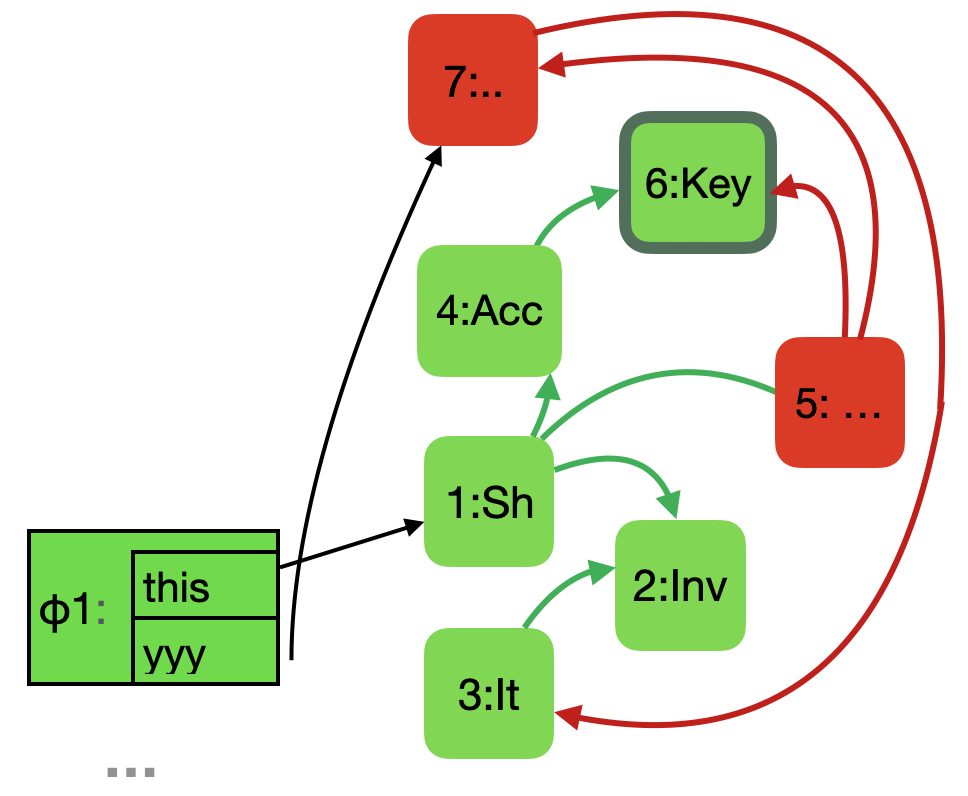
\includegraphics[width=\linewidth]{diagrams/ShopB.png}
} 
&
\resizebox{3,5cm}{!}{
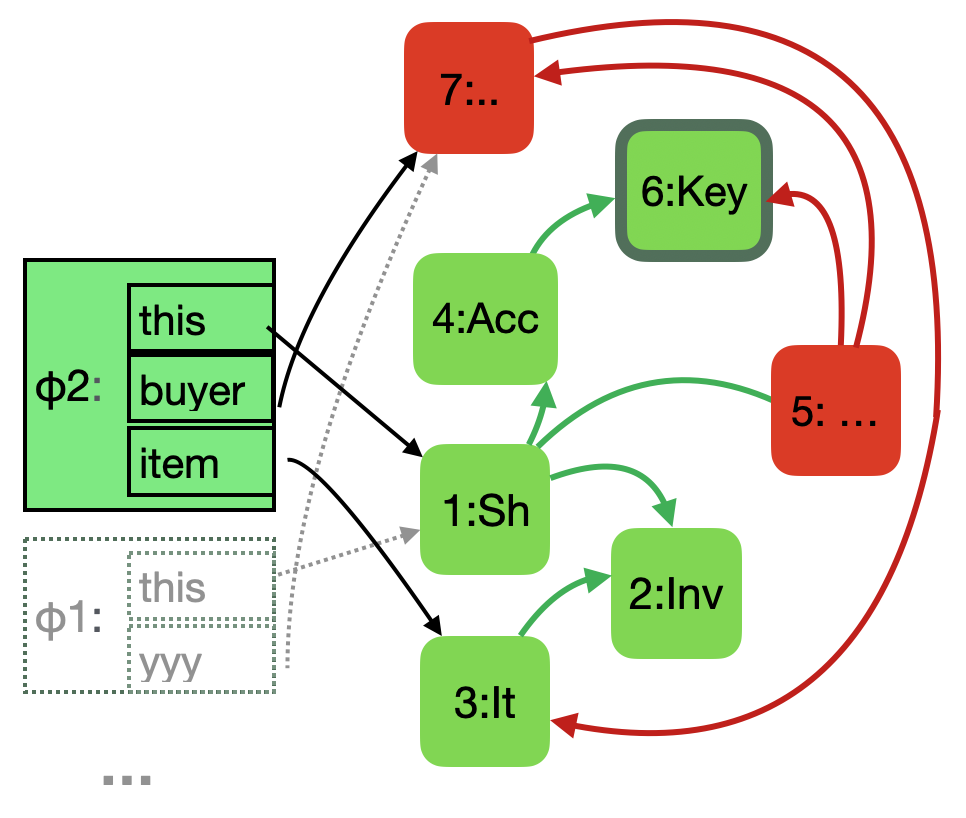
\includegraphics[width=\linewidth]{diagrams/ShopC.png}
}
&
\resizebox{3.5cm}{!}{
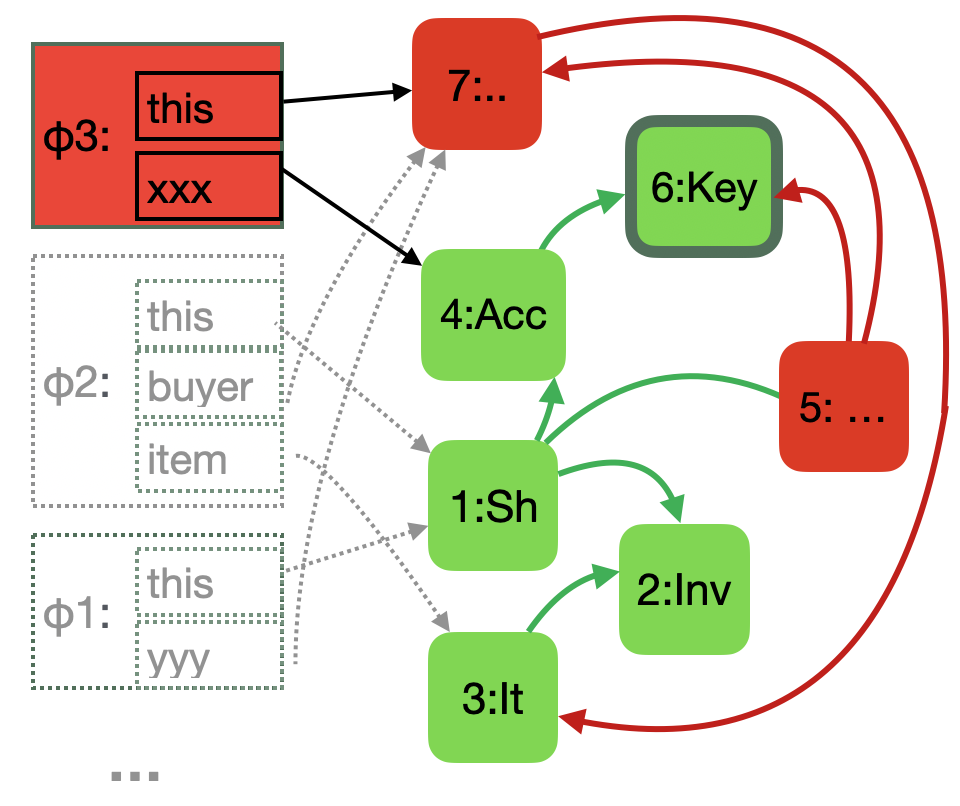
\includegraphics[width=\linewidth]{diagrams/ShopD.png}
}
\\
\hline
$\sigma_1$, top frame $\phi_1$  % protected from object $o_2$
&
$\sigma_2$, top frame $\phi_2$ 
&
$\sigma_3$, top frame $\phi_3$ 
\\
\hline % \hline
\end{tabular}
\caption{\textit{The current point of execution} before \prg{buy}, during \prg{buy}, and during \prg{pay}.  Frames $\phi_1$, $\phi_2$ are green  as their receiver (\prg{this}) is internal;  $\phi_3$ is red as its receiver is external. Continuations are omitted.}
 \label{f:CurrentPoint}
 \end{figure}


\subsubsection{Protection}
\label{sect:approach:protection}


 \begin{description}
\item[Protection] 
Object $o$ is \emph{protected  from} object $o'$, formally $\protectedFrom {o} {o'}$,  
% SD: I added "object" in the sentence above, because otherwise the symbol for protection looked funny
if no external object indirectly accessible from $o'$ has direct access to $o$.
Object $o$ is \emph{protected}, formally ${\inside{\prg{\it{o}}}}$,  
if no external object indirectly accessible from the current frame has direct access to $o$,
 and  if the receiver is external then $o$ is not an argument.\footnote{An object has direct access to another object if it has a field pointing to the latter;
 it has indirect access to another object if there exists a sequence of field accesses (direct references) leading to the other object; 
 an object is indirectly accessible from the frame if one of the frame's variables has indirect access to it.} 
 More in Def.\ \ref{def:chainmail-protection-from}.   
\end{description}
 
 
Fig.\ \ref{fig:ProtectedBoth} illustrates \emph{protected} and \emph{protected
from}. Object $o_6$ is not protected in states $\sigma_1$ and
$\sigma_2$, but \emph{is} protected in state $\sigma_3$.
This is so, because the external object $o_5$ is indirectly accessible from the top frame in $\sigma_1$ and in  $\sigma_2$, but not
from the top frame in $\sigma_3$ --
in general, calling a method (pushing a frame) can only ever \emph{decrease} the set of indirectly accessible objects. 
Object $o_4$  is  protected in  states $\sigma_1$ and  $\sigma_2$,  and not  protected in state $\sigma_3$
because though neither object $o_5$ nor $o_7$ have direct access to $o_4$, in state $\sigma_3$ the receiver is external and $o_4$ is one of the arguments.

 
\begin{figure}[htb]
\begin{tabular}{|c|c|c|c|}
\hline
 heap
&
$\sigma_1$   
&
$\sigma_2$ 
&
$\sigma_3$ 
\\
\hline 
$... \models \protectedFrom {o_6} {o_4}$
&
$\sigma_1   \not\models \inside{o_6}$
&
$\sigma_2   \not\models \inside{o_6}$
&
$\sigma_3 \models \inside{o_6}$
\\
$... \not\models  \protectedFrom {o_6} {o_5}$
&
$\sigma_1  \models \inside{o_4}$
&
$\sigma_2 \models \inside{o_4}$
&
$\sigma_3 \not \models \inside{o_4}$
\\
\hline  
\end{tabular}
\caption{\textit{Protected from and Protected}. -- continuing from Fig, \ref{f:CurrentPoint}.
 }
   \label{fig:ProtectedBoth}
 \end{figure}

If a protected object $o$ is never passed to external objects (\ie never leaked)  then $o$ will remain protected during the whole execution of the current method,
including during any nested calls.
% and all the methods \emph{it} calls. 
This is the case even if $o$ was not protected before the call to the current method.
% Moroever,  during the remainder of the execution of the method calling the current method, nor after termination of the current method.
We define  \emph{scoped invariants} to  describe 
% was such  guarantees that properties are preserved within the current call and all nested calls.
%\sdnew
{property  preservation within the current  and all its nested calls}.



 

\subsubsection{Scoped Invariants}
 
\label{sect:approach:scoped}
We build on the concept of history invariants \cite{liskov94behavioral,usinghistory,Cohen10} and define:

\begin{description}
\item[{Scoped invariants}]  
{$\TwoStatesN  {\overline{x:C}}  {A}$} expresses that if an external {state} $\sigma$ 
 has objects $\overline x$ of class $\overline C$, and satisfies $A$, then all  {external} states which are part of
the \emph{scoped  future} of $\sigma$   will  {also} satisfy  {$A$}. 
The scoped future contains all  states which can be reached through any program execution steps, including further method calls and returns, but stopping just before returning  from the call active in $\sigma$ \footnote{{Here lies the difference to history invariants, which consider \emph{all} future states, including returning from the call active in $\sigma$.}}  --  \cf Def  \ref{def:shallow:term}.
% {For} $\sigma$ and its scoped future we 
% Scoped invariants only consider external states -- \cf Def \ref{def:necessity-semantics}.
\end{description}


Fig.\ \ref{fig:illusrPreserve} shows the  states of an unspecified execution starting at internal state $\sigma_3$ and terminating at internal state $\sigma_{24}$.
% Fig.\ \ref{fig:illusrPreserve} 
It distinguishes between steps within the same method ($\rightarrow$),
method calls ($\uparrow$), and method returns ($\downarrow$). %  method; up-arrows represent ; down-arrows represent method returns.
The scoped future of $\sigma_6$ consists of $\sigma_6$-$\sigma_{21}$, but does not contain $\sigma_{22}$ onwards, since  scoped future stops before returning. 
  Similarly, the scoped future of $\sigma_9$ consists of $\sigma_9$, $\sigma_{10}$,  $\sigma_{11}$,  
  $\sigma_{12}$,   $\sigma_{13}$,  and $\sigma_{14}$, and does not include, \eg,  $\sigma_{15}$, or $\sigma_{18}$.
 
\begin{figure}[htb]
\begin{tabular}{|c|}
\hline  % \\
\hspace{2cm}
%\resizebox{7.6cm}{!}{
\resizebox{9cm}{!}{
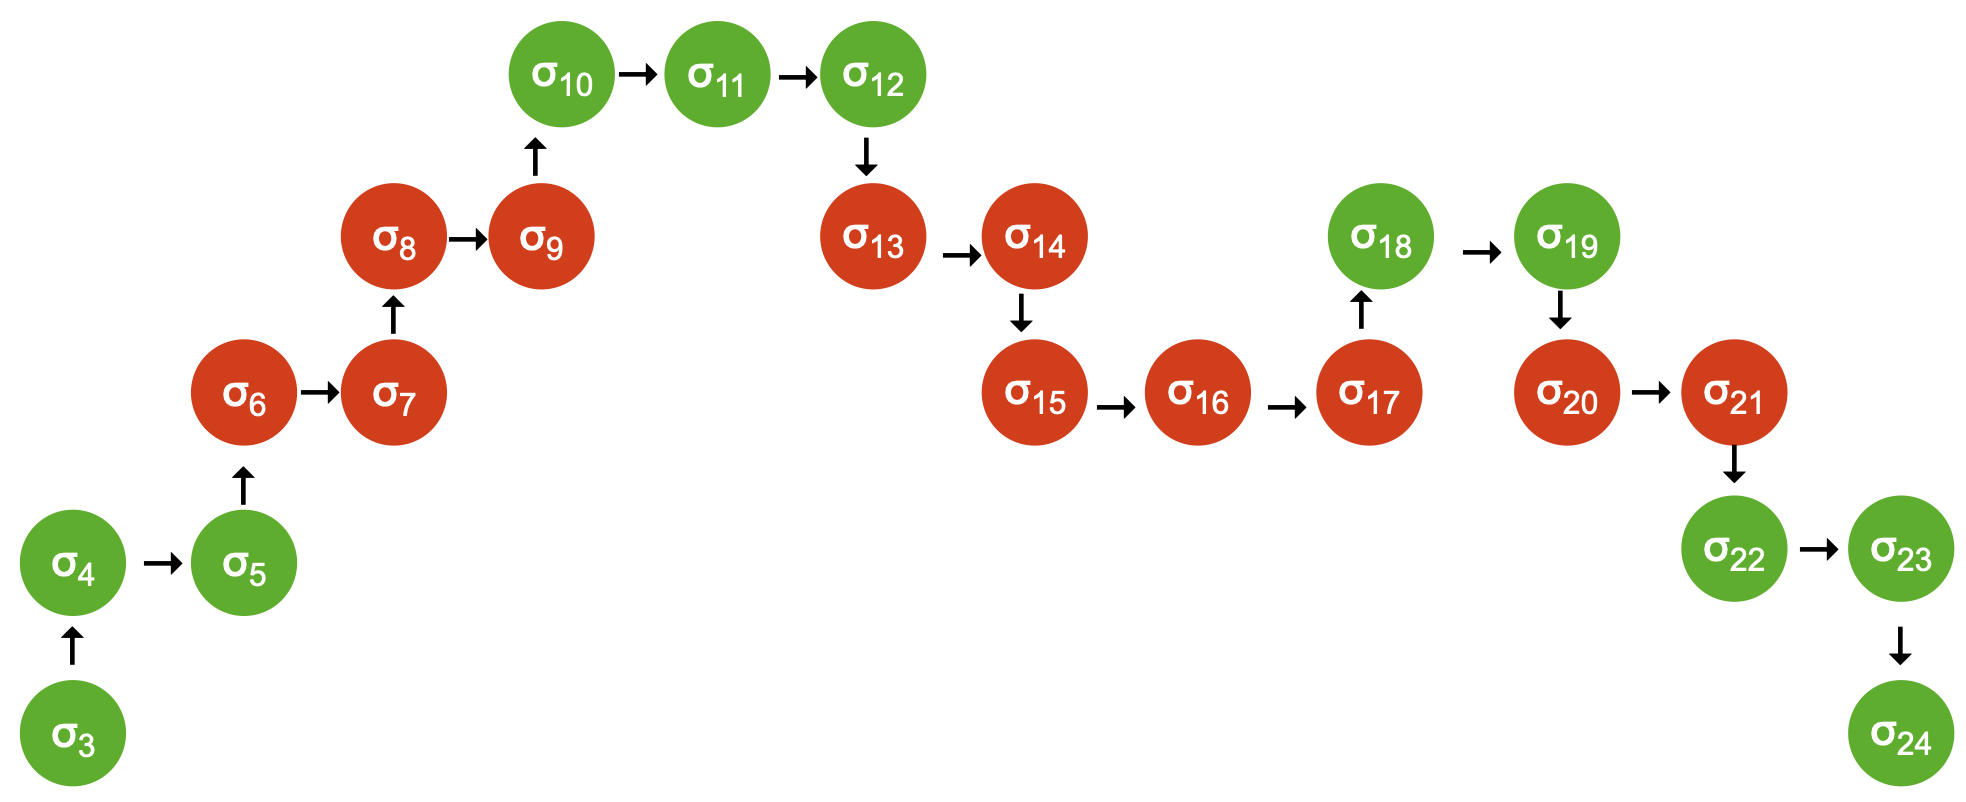
\includegraphics[width=\linewidth]{diagrams/executionDisks.png}  % diagrams/preserves2.png} is same but with pink external states
}
\hspace{2cm}
\\
\hline
\end{tabular}
   \caption{ \textit{Execution}.
Green disks represent internal states; red disks external states.
}
 \label{fig:illusrPreserve} 
 \end{figure}
 
The scoped invariant   ${\TwoStatesN {\overline {x:C}} {A_0}}$   guarantees that  if $A_0$ holds in $\sigma_8$, then it will also hold in $\sigma_9$,    $\sigma_{13}$, and $\sigma_{14}$;
 it   doesn't have to hold in $\sigma_{10}$, $\sigma_{11}$,  and $\sigma_{12}$ as these are internal states.
 Nor does it have have to hold at $\sigma_{15}$ as it is not part of $\sigma_9$'s scoped future.
%Similarly, it guarantees that if $A_0$ holds at $\sigma_6$, then it will also hold at 
%$\sigma_7$, $\sigma_8$, $\sigma_9$, $\sigma_{13}$,  $\sigma_{14}$,   $\sigma_{15}$,  $\sigma_{16}$, $\sigma_{17}$,   $\sigma_{20}$ and  $\sigma_{21}$; it may or may not hold at
%$\sigma_{10}$, $\sigma_{11}$,  $\sigma_{12}$,  $\sigma_{18}$,  $\sigma_{19}$, as these are internal states.


 

% \subsubsection{Examples}    
    
\label{s:bank}

\begin{example}
\label{s:bankSpecEx}
The following scoped invariants\\
$\strut \SPSP\ \ \   S_1\ \  \triangleq \ \ \TwoStatesN {\prg{a}:\prg{Account}}  {\inside{\prg{a}}} $ 
\hspace{1.1cm}
$\strut  \SPSP\ \ \   S_2\ \  \triangleq \ \ \TwoStatesN  {\prg{a}:\prg{Account}}  {\inside{\prg{a.key}}} $ 
% \\
%$\strut  \SPSP   S_3\ \  \triangleq \ \ \TwoStatesN {\prg{a}:\prg{Account},\prg{b}:\prg{int}}  {\inside{\prg{a}} \wedge \prg{a.\balance}=\prg{b}}  $
\\
$\strut  \SPSP\ \ \   S_3\ \  \triangleq \ \ \TwoStatesN{ \prg{a}:\prg{Account},\prg{b}:\prg{int} } {\inside{\prg{a.key}} \wedge \prg{a.\balance} \geq \prg{b} } $ 
% \end{tabular}
%}

\noindent
%specifications
 guarantee that   accounts are not leaked  ($S_1$), \ \ keys are not leaked  ($S_2$), \ \  and that the balance does not decrease unless there is unprotected access to the key  ($S_3$).
 % $\strut  \SPSP  S_1$:\   accounts are not leaked,  \hspace{1.1cm}
%$\strut   \SPSP S_2$:\    keys are not leaked,\\
%%$\strut \SPSP  S_3$:\  the balance is not modified unless there is unprotected access to the account,  \\%while 
%$\strut \SPSP  S_3$:\   the balance does not decrease unless there is unprotected access to the key.  
%
\end{example} 
% \vspace{.005cm}

 
\noindent
This example illustrates three crucial properties of our invariants:
 \begin{customquote}
 \vspace{.05cm}
\noindent
\textbf{\emph{Conditional}}: They %Invariants 
are \emph{preserved}, but unlike object invariants, they do not % guarantee that they
always hold.
\ \Eg   \prg{buy} cannot assume $\inside{a.\prg{key}}$ holds on entry, but   guarantees that if it holds on entry, then  it will still hold on exit.

\vspace{.05cm}
\noindent
\textbf{\emph{Scoped}}:  %  These invariants 
They % Invariants
 are preserved during  execution of a specific method but not beyond its return. It is, in fact, expected that the invariant will eventually cease to hold after its completion. For instance, while $\inside{a.\prg{key}}$ may currently hold, it is possible that an earlier (thus quiescent) method invocation frame has direct access to $a.\prg{key}$ -- without such access, $a$ would not be usable for payments. Once control flow returns to the quiescent method (\ie enough frames are popped from the stack) $\inside{a.\prg{key}}$  will no longer hold.

 \vspace{.05cm}
\noindent
\textbf{\emph{Modular}}: They % Invariants 
describe  externally observable effects (\eg  \prg{key} stays protected) across whole modules,
 % the account's balance may increase), 
rather than  the individual methods (\eg\, \prg{set}) making up a module's interface.
Our example specifications will
%  or \prg{transfer})
characterize \emph{any}
module defining accounts with a  % {\textit{implementation}} of a bank account with a 
 \balance~and a \prg{\password} -- even as ghost fields --  irrespective of their APIs. % offered. -- short
 \end{customquote}
 
 \begin{example}
 We   now use the features from the previous section to specify methods. 

{\sprepostShort
		{\strut \ \ \ \ S_4} 
		{   \protectedFrom{\prg{this}.\prg{\myAccount}.\prg{key}} {\prg{buyer}} \wedge \prg{this}.\prg{\myAccount}.\prg{\balance}=b
		 }
		{\prg{public Shop}} {\prg{buy}} {\prg{buyer}:\prg{external}, \prg{anItem}:\prg{Item} }
		{ 
		  %\protectedFrom{\prg{this}.\prg{\myAccount}.\prg{key}} {\prg{buyer}} \wedge 
		  \prg{this}.\prg{\myAccount}.\prg{\balance}\geq b
		} 
		}

\noindent
$S_4$  guarantees that if the  key was protected from \prg{buyer} before the call, then the balance will not decrease\footnote{We ignore the ... for the time being.}.
 It does \emph{not} guarantee \prg{buy} will only be called when $\protectedFrom{\prg{this}.\prg{\myAccount}.\prg{key}} {\prg{buyer}}$ holds: 
as a  public method,  \prg{buy}  can be invoked by external code that ignores all specifications.
\end{example}

% \vspace{.05cm}

\begin{example}
\label{e:versions}
We illustrate the meaning of our specifications using three versions 
($\ModA$,  $\ModB$, and $\ModC$) of the \Mshop module \cite{OOPSLA22};
these all share the same \prg{transfer} method to withdraw money: 

\begin{lstlisting}[mathescape=true, language=Chainmail, frame=none]
module $\ModA$      
  class Shop   ... as earlier ...
  class Account
    field blnce:int 
    field key:Key
    public method transfer(dest:Account, key':Key, amt:nat)
       if (this.key==key')  this.blnce-=amt; dest.blnce+=amt
    public method set(key':Key)
       if (this.key==null)  this.key=key'
\end{lstlisting}

\noindent Now consider modules \ModB and \ModC, which differ from \ModA
only in their \prg{set} methods. Whereas \ModA 's key is fixed once it is \prg{set},
%can be assigned once and not changed subsequently
\ModB allows any client to \prg{set} an account's key at any time, while
%\ModC requires the existing key in order to reset it.
\ModC requires the existing key in order to replace it.

\vspace*{2mm}

\begin{tabular}{lll}
\begin{minipage}[b]{0.40\textwidth}

\begin{lstlisting}[mathescape=true, language=Chainmail, frame=none]
module $\ModB$
  ... as earlier ...
  public method set(key':Key)
    this.key=key'
\end{lstlisting}
\end{minipage}
&\ \ \  \ \   &%
\begin{minipage}[b]{0.48\textwidth}
\begin{lstlisting}[mathescape=true, language=chainmail, frame=none]
module $\ModC$
  ... as earlier ...
  public method set(key',key'':Key)
    if (this.key==key')  this.key=key''
\end{lstlisting}
\end{minipage} 
\end{tabular}

Thus, in all three modules, the key is a capability which \emph{enables} the withdrawal of the money. 
Moreover, in $\ModA$ and $\ModC$, the key capability
%{is a capability} used to  \emph{tame} withdrawal of money, 
is a necessary precondition for withdrawal of money, while in % preventing those without it from getting the money from the account.}
 in $\ModB$ it is not. % the key \emph{does not tame} withdrawal of money.
Using $\ModB$, it is possible to start in a state where the account's key is unknown, modify the key, and then withdraw the money. 
Code   such as 
\\ 
$\ \strut \hspace{.2in} $ \prg{k=new Key;  acc.set(k); acc.transfer(rogue\_accnt,k,1000)} 
\\ 
is enough to drain  \prg{acc} in \ModB without knowing the \password.\footnoteSD{CAREFUL: we had 
$\ \strut \hspace{.01in} $ \prg{an\_account.set(42); an\_account.transfer(rogue\_accnt,42)} but this was type incorrect!}
% \emph{Emergent behaviour} is key here: 
Even though  \prg{transfer} in  \ModB is ``safe'' when considered in isolation, it is not safe when considered in conjunction with other methods from the same module. 

%Modules 
$\ModA$ and $\ModC$ satisfy $S_2$ and $S_3$, while $\ModB$ satisfies neither. 
So if $\ModB$ was required to satisfy either $S_2$ or $S_3$ %and the programmer wrote version $\ModB$, it 
then it would  be rejected by our inference system as not safe.
None of the three versions satisfy $S_1$ because \prg{pay}  could leak %leaks 
an \prg{Account}.

\end{example}
 
% , services  exported, or  dependencies on other parts of the system.\footnoteSD{does this come from OOPSLA? if so we need to rephrase}
%\notesep
%Adherence to   specifications is not monotonic:
%{Eg, while  \ModA satisfies $S_3$, the addition of \prg{set} lead to \ModB, which does not.}
%% Adding a method to a module does not necessarily preserve such adherence,
%% \eg adding method \prg{set} in module \ModB breaks 
%%SD removed the below. When we changed the invaraints to have the same assertion re and post it no longer hel
%\forget{, and while separate methods may adhere to a  specification, their combination does
%not necessarily do so. 
%{For example, \ModB's  \prg{tansfer} and \prg{set} satisfy $S_3$, but their interplay does not.}
%%In this sense, and, similar to OOPSLA'22, our  specifications capture a module's \emph{emergent behaviour}. 


  
  \subsection{2$^{nd}$ Challenge:  A Hoare logic for adherence to specifications}  
 \label{sec:howSecond}

\paragraph{Hoare Quadruples} Scoped invariants require quadruples, rather than  classical triples.
Specifically, \\
  $\strut \ \hspace{4cm} {\TwoStatesN  {\overline{x:C}}  {A}}$\\
 asserts that if an external {state} $\sigma$ 
 satisfies  $\overline {x:C} \wedge A$, then all its \emph{scoped} external future  states will   also  satisfy  $A$. 
For example, if $\sigma$ was an external state executing a call to \prg{Shop::buy}, then a \emph{scoped} external future  state
 %could be the external state  after  return from \prg{Shop::buy}, or 
 could be reachable during execution of the   call \prg{pay}.
This implies that we consider not only states at termination but also external states reachable
 \emph{during} execution of  statements. 
To  capture this, we extend   traditional Hoare triples to quadruples of  form\\
 $\strut \ \hspace{4cm} \quadruple {A} {\, stmt\, }{A'} {A''}$\\  
 promising that if a state satisfies $A$ and executes $stmt$, any terminating state will satisfy $A'$, and 
 and  any intermediate external states reachable during execution of $stmt$ satisfy    $A''$ -- \cf Def. \ref{def:hoare:sem}.
 
\vspace{.1cm}

We assume an  underlying   Hoare logic  of  triples  
$ M \vdash_{ul} \{ \ A\ \} {\ stmt\ }\{\ A'\ \} $,
which does not {have} the concept of protection -- %  and does not deal with external calls. 
that is, the assertions $A$ in the $\vdash_{ul}$-triples do not mention protection.
%, and $stmt$ does not contain external calls.
We then embed  the $\vdash_{ul}$-logic into the quadruples logic 
( $\vdash_{ul}$-triples  whose   statements do not contain method calls give rise to quadruples in our logic -- see rule below).
We  extend assertions $A$ so they may mention protection and add rules about protection
 (\eg newly created objects are protected -- see rule below), and
 add   usual conditional and substructural rules.
 More in Fig.\ref{f:protection}  and \aref{Fig. 15}{\ref{f:substructural:app}}.

\noindent
\small
\noindent
\begin{center}
$  
\begin{array}{lcr}
\inferruleNoName 
	{  
	  M \vdash_{ul} \{ \ A\ \} {\ stmt\ }\{\ A'\ \}   \ \ \ \ stmt\  \mbox{calls no methods}  %or 'makes no calls`
	}
	{\hprovesN{M}  {A} {\ stmt \ } {A'} {A''} } 
&   &
\inferruleNoName 
	{ 
	 	
	}  	 
	{	 
 	\hprovesN  {M}  
	                {  true  }  
 			   {\  u = \prg{new}\ C \ }
 			   {\  \inside{u}\  }  { \ A \ }
	}
%& &
%\inferruleNoName 
%	{
%	 M \vdash_{ul} \{ \ A\ \} {\ stmt\ }\{\ A'\ \} 
%	}  
%	{ \hproves  {M}  {A} {\ stmt\ }{A'} }
\end{array}
$
\end{center}

\normalsize

%\vspace{.1cm}
\paragraph{Well-formed modules and External Calls} A module is well-formed, if  its specification is well-formed,   its public methods preserve   the module's scoped invariants, and  all  methods satisfy their specifications - \cf  Fig.  \ref{f:wf}.
%A well-formed  specification  does not mention protection in negative positions (this is needed for the soundness of the method call rules). 
%A method satisfies  scoped invariants (or method  specification) if its body satisfies the relevant pre- and post-conditions.
%\Eg to prove  that  \prg{Shop::buy} satisfies {$S_3$}, taking   $stmts_{b}$ % $stmt\_{buy}$   is 
%for the    body of \prg{buy},  we  have to prove:
%\sdnew
{\Eg to prove  that  \prg{Shop::buy} satisfies {$S_4$}, taking   $stmts_{b}$ % $stmt\_{buy}$   is 
for the    body of \prg{buy},  we  have to prove:}
\\
% this is for the other methods
%$\strut \ \ \ \ \ \ \ \ \ \ \ \quadruple {A_1  \wedge \inside{\prg{a}} } {\ stmt\_b  \ } {\inside{\prg{a}}} { \inside{\prg{a}}} $
%\\
%$\strut \ \ \ \ \ \   \ \  \quadruple {A_1  \wedge  \inside{\prg{a.\password}} } {\  stmt\_buy  \  } {\inside{\prg{a.\password}}}  {\inside{\prg{a.\password}}}$
%\\
%$\strut \ \ \ \ \ \  \ \  \ \ \   \quadruple {A_1  \wedge  \inside{\prg{a.key}} \wedge  \prg{a.\balance}\!=\!{\prg{b}} } {\   stmt\_b  \  } {\inside{\prg{a.key}} \wedge  \prg{a.\balance}\!=\!\prg{b}}   
%                         {  \inside{\prg{a,key}} \wedge  \prg{a.\balance}\!=\!\prg{b} }$
%\\
%$\strut \ \ \ \ \ \   \ \   \quadruple {A_0  \wedge  \inside{\prg{a.\password}} \wedge  \prg{a.\balance}\!\geq\!{\prg{b}} } {\  stmts_{b}  \  } {\inside{\prg{a.\password}} \wedge  \prg{a.\balance}\!\geq\!{\prg{b}}}  
%   { \inside{\prg{a.\password}}\wedge  \prg{a.\balance}\!\geq\!{\prg{b} }}$
%}}
%\\
%and similar for {$S_3$}. 
% Here we used   
% \small
%$
%\begin{array}{ll}
%\ \ \ \ \  &   
%                     \{ \ {A_0  \wedge  \inside{\prg{a.\password}} \wedge  \prg{a.\balance}\!\geq\!{\prg{b} } } \  \} \\
%		& \ \ \ \ \ \ \ \ \ \   stmts_{b} \  \\
%		&
%                   \{\  {\inside{\prg{a.\password}} \wedge  \prg{a.\balance}\!\geq\!{\prg{b}} }  \ \}\ \  ||\ \  \{\ \inside{\prg{a.\password}}\wedge  \prg{a.\balance}\!\geq\!{\prg{b}}   \ \} 
%\end{array}
%$
%\\
%\noindent 
% where $A_0 \triangleq $ %  {\small{
%\prg{this}:\prg{Shop}, \prg{buyer}:\prg{external}, \prg{anItem}:\prg{Item}, \prg{a}:\prg{Account},  \prg{b}:\prg{int}.
%
%
\sdnew{ \vspace{.05cm}
  \begin{minipage}{.05\textwidth}
   \textbf{(0)}\ \ 
\end{minipage}
\hfill
\begin{minipage}{.95\textwidth}
\begin{flushleft}
$\{\  \   \external{\prg{buyer}} \ \wedge\ 
% red here is meanrt to make the contrast with the  next one 
  \protectedFrom {\prg{this.\myAccount.key}} {\prg{buyer} } 
 \ \wedge\ \prg{this.\myAccount.\balance}= b  \ \  \}$\\
$\ \ \ \ \ \ \ \ \ \ \ \ {\ \ stmts_{b}   \ } $\\
$  \{\  \ \  {\prg{this.\myAccount.\balance}} \geq  b \  \  \} \ \ ||\ \  \{ \ ... \ \} $ % \{\ \inside{\prg{a.\password}}\wedge  \prg{a.\balance}\!\geq\!{\prg{b}}   \ \}  $  simpler
\end{flushleft}
\end{minipage}
}
%\\
%\noindent
%which says that  if the shop's account's key is protected from \prg{buyer}, then the account's balance will not decrease after 
%execution of \prg{buy}.


 
 \label{sec:howThird}
% \paragraph{External Calls}  

\sdnew{The proof} %that a method body satisfies pre- and post-conditions 
\sdnew{proceeds using}   %\sdnew
{our Hoare quadruples logic}. % discussed in this section.
The treatment of external calls is of special interest. 
% For example,   % consider  the 
%  \sdnew{for the proof of  \textbf{(0)}}, %verification of $S_4$. 
%\sdnew
{Here,} the challenge is % how to reason  about 
the external call \sdnew{on line 8}. % (from \prg{buy} in \prg{Shop}). 
We need to establish the Hoare quadruple:

 \vspace{.05cm}
  \begin{minipage}{.05\textwidth}
   \textbf{(1)}\ \ 
\end{minipage}
\hfill
\begin{minipage}{.95\textwidth}
\begin{flushleft}
$\{\  \   \external{\prg{buyer}} \ \wedge\ 
% red here is meanrt to make the contrast with the  next one 
 {\color{red} {\protectedFrom {\prg{this.\myAccount.key}}  {\prg{buyer} } }}
 \ \wedge\ \prg{this.\myAccount.\balance}= b  \ \  \}$\\
$\ \ \ \ \ \ \ \ \ \ \ \ {\ \prg{buyer.pay(this.accnt,price)}   \ } $\\
$  \{\  \ \  {\prg{this.\myAccount.\balance}} \geq  b \  \  \} \ \ ||\ \  \{ \ ... \ \} $ % \{\ \inside{\prg{a.\password}}\wedge  \prg{a.\balance}\!\geq\!{\prg{b}}   \ \}  $  simpler
\end{flushleft}
\end{minipage}
\\
\noindent
which says that  if the shop's account's key is protected from \prg{buyer}, then the account's balance will not decrease after the call \sdnew{of
\prg{pay}.}
 \vspace{.05cm}
 
To prove \textbf{(1)}, we aim to use $S_3$, but this is not straightforward: %Applying
 $S_3$  requires 
 % the red here is intended to make the contrast with the provious one
 {\color{red} {$\inside{\prg{this.\myAccount.key}}$}}, 
 which is not provided by the precondition of \textbf{(1)} .
 % only provides $\protectedFrom{\prg{this.\myAccount.key}}{\prg{buyer}}$. And 
 More alarmingly,  
$\inside{\prg{this.\myAccount.key}}$ may \emph{not hold} at the time of the call.
%
For example, in state $\sigma_2$ (Fig. \ref{fig:ProtectedBoth}), which could initiate the call to \prg{pay}, we have $\sigma_2 \models \protectedFrom{o_4\prg{.key}} {o_7}$, but $\sigma_2 \not\models \inside{o_4\prg{.key}}$.

Fig. \ref{fig:ProtectedBoth} provides insights into addressing this issue. Upon entering the call, in state $\sigma_3$, 
we find that $\sigma_3 \models \inside{o_4\prg{.key}}$. More generally, if $\protectedFrom{\prg{this.\myAccount.key}}{\prg{buyer}}$ holds before the call to \prg{pay}, then $\inside{\prg{this.\myAccount.key}}$ holds upon entering the call.
This is because any objects indirectly accessible during \prg{pay} must have been indirectly accessible from the call's
receiver (\prg{buyer}) or  arguments (\prg{this.\myAccount} and \prg{price}) when \prg{pay} was called.
% The below is true but is not sufficient reason why <<this.accnt.key>> inside the call.
% --- calls cannot increase the set of indirectly accessible objects (\S \ref{sect:approach:protection}).
 
In general, if   $\protectedFrom{\prg{x}}{\prg{y}_i}$ holds  for all %arguments 
 $\prg{y}_i$, before a call $\prg{y}_0.m(\prg{y}_1, ..., \prg{y}_n)$, then $\inside{\prg{x}}$ holds  upon entering the call. 
% chopped as adaptation not as prominent
%To formulate this, we introduce the adaptation operator $\pushSymbolInText$, which translates assertions from the caller's perspective to that of the callee. 
%Specifically, $\PushASLong  {(\prg{y}_0, ..., \prg{y}_n)}   A$ at a call, ensures   $A$  when the variables  $\prg{y}_0, ..., \prg{y}_n$ are pushed onto a new frame. More in Def   \ref{def:push} and  Lemma \ref{lemma:push:ass:state}. Here, \\
%$\strut \ \ \ \ $  \small $\PushASLong {(\prg{buyer},\prg{this.\myAccount},\prg{price})} {\inside{\prg{this.\myAccount.key}}}$
%= $\protectedFrom{\prg{this.\myAccount.key}}{\prg{buyer}}$\\
%  \normalsize 
Here we have  $\protectedFrom{\prg{this.accnt.key}}{\prg{buyer}}$ by precondition. We also  have that \prg{price} is a scalar and therefore 
$\protectedFrom{\prg{this.accnt.key}}{\prg{price}}$.  And the type information gives that
all fields transitively accessible from an \prg{Account} are scalar or internal; this gives that
$\protectedFrom{\prg{this.accnt.key}}{\prg{this.accnt}}$. 
This enables the application of $S_3$ in \textbf{(1)}. The corresponding Hoare logic rule is shown in Fig. \ref{f:external:calls}.

% {Below  a  Hoare logic rule  dealing with external calls - \cf. Fig.\ref{f:external:calls}.} % where $\overline y$ stands for $y_1$,...$y_n$ -
% 
% \begin{minipage}{.05\textwidth}
%   \textbf{(2)}
%\end{minipage}
%\hfill
%\begin{minipage}{.95\textwidth}
%\begin{flushleft}
% $\inferruleNoName  
% 	{ 
%   	   {\TwoStatesN {\overline {x:D}} {A}}\ \   \mbox{is part of $M$'s specification}
%        }
%	{    \hprovesN{M} 
%						{ \    { \external{y_0}} \,     \wedge \,  \overline{x:D}\  \wedge\ {\PushASLong {{(y_0,\overline {y})}}  {A}}  \ } 
%						{ \ u:=y_0.m(y_1,.. y_n)\    }
%						{ \   {\PushASLong {{(y_0,\overline {y})}}  A}  \ }
%						{\  A \   }         }
%$
%\end{flushleft}
%\end{minipage}
%
%\vspace{.05cm}
%%  \noindent
%To prove  \textbf{(1)},  we take \  $y_0 \triangleq \prg{buyer}$,\ \ \  $\overline {x : D}\triangleq \prg{a}:\prg{Account},\prg{b}:\prg{int}$, 
%\ \ $A \triangleq  \inside{\prg{a.\pwd}}\wedge \prg{a.\balance}\geq \prg{b}$, \ \ 
%$m \triangleq \prg{pay}$,\ and $\overline {y} \triangleq \prg{this.accnt},\prg{price}$. 
%% \\
% Moreover, $\PushAS y {\inside \re} = \protectedFrom \re {\overline{y}}$ for any term $\re$ and variables $\overline y$ 
%-- see  Def. \ref{def:push}.
%Therefore:\\
%   {\small{$\strut \ \ \ \PushASLong {(\prg{buyer},\prg{this.\myAccount},\prg{price})}  {\inside {\prg{this.\myAccount.key}}}$}} \ = \\
%%    \begin{flushright}
% {\small{$\strut \ \hspace{5.5cm}  \protectedFrom {\prg{this.\myAccount.key}} {(\prg{buyer},\prg{this.\myAccount},\prg{price})}$}}.\\
%% \end{flushright}
% The type information gives:\\
%  {\small{$\strut \ \ \ \protectedFrom {\prg{this.\myAccount.key}} {\prg{this.\myAccount}}\ = true \ =  \protectedFrom {\prg{this.\myAccount.key}} {\prg{price}}$}}\\
%  Hence\\
%  {\small{$\strut \ \ \ \protectedFrom {\prg{this.\myAccount.key}} {(\prg{buyer},\prg{this.\myAccount},\prg{price})}$ 
% \ = \  $\protectedFrom {\prg{this.\myAccount.key}} {\prg{buyer}}$.}} \\
%We use the above,  apply the external method call rule \textbf{(2)},  and obtain \textbf{(1)}.
% %
 

 
\subsection*{Summary}

In  an open world, external objects can execute arbitrary code, invoke any public internal methods, access any other external objects, and even collude with each another.
The external code may be written in the same or a different programming language than the internal code -- all we need is that the platform protects direct external read/write of  the internal private fields, while allowing indirect manipulation through calls of public methods.

 

The conditional and scoped nature of our invariants is critical to their applicability.
%might prompt questions about their usefulness.
Protection is a local condition, constraining accessible objects rather than imposing a structure across the whole heap.
Scoped invariants are likewise local: they do not preclude some effects from the whole execution of a program,
rather the effects are precluded only in some local contexts.
%take place in contexts where specified conditions are satisfied.
While $a.\prg{\balance}$ may decrease in the future, this can only happen in contexts where an external object has direct access to  $a.\prg{key}$. 
Enforcing these local conditions is the responsibility of the internal module:
precisely because these conditions are local, they can be enforced locally within a module,
irrespective of all the other modules in the open world.
 % something good does hold. 
 % Nevertheless, they do give the guarantee that something good does not get broken.
 
 
%% The key ingredients of our work are: \ \ the concepts of protection ($\inside {x}$ and $\protectedFrom {x} {y}$),\ \  \scoped invariants (${\TwoStatesN {\overline {x:D}} {A}}$), \ \  and  the adaptation operator ($\FIXSymbolA$).
%%  In the remaining sections we discuss all this in more detail.
 

